
\documentclass[10pt,a4]{article}
\usepackage[english]{babel}
\usepackage[utf8x]{inputenc}
\usepackage{amsmath}
\usepackage{graphicx}
\usepackage[colorinlistoftodos]{todonotes}
\usepackage{hyperref}
\usepackage{geometry}
\usepackage{float}
\usepackage{xkeyval}
\usepackage[export]{adjustbox}
\geometry{top=3cm,left=2cm,right=2cm,bottom=3cm}
\usepackage[scaled]{helvet}
\usepackage[T1]{fontenc}
\renewcommand\familydefault{\sfdefault}
\newcommand{\code}[1]{\texttt{#1}}


\author{Ottavia Belotti\quad Riccardo Izzo}
\date{\today}
\title{Publisher/Subscriber IPC}



\begin{document}
\maketitle
\tableofcontents

\section{Project data}

\begin{itemize}
\item 
  Project supervisor(s): Federico Reghenzani

\item 
Project team:

\begin{center}
\begin{tabular}{lll}
Last and first name & Person code & Email address\\
\hline
  Belotti Ottavia & 10657411 & ottavia.belotti@mail.polimi.it \\
  Izzo Riccardo & 10599996 & riccardo.izzo@mail.polimi.it                     
\end{tabular}
\end{center}

\item
Subdivision of development tasks:\\
\textbf{Ottavia Belotti}:
\begin{itemize}
  \item subscriber\_write: write function for subscribe device file
  \item signal\_nr\_write: write function for signal\_nr device file
  \item endpoint\_write: write function for endpoint device file
  \item permissions of device files
  \item concurrency
\end{itemize}

\textbf{Riccardo Izzo}:
\begin{itemize}
  \item new\_topic\_write: write function for new\_topic device file
  \item release\_file: function that release all the device files when unloading the module
  \item subs\_list\_read: read function for subscribers\_list device file
  \item endpoint\_read: read function for endpoint device file
  \item ownership of device files
\end{itemize}

\item Links to the project source code: \url{https://github.com/RiccardoIzzo/AOS-Publisher-Subscriber-IPC}

\end{itemize}


\section{Project description}

\begin{itemize}
\item What is your project about?\\
The project consists in the implementation of a Linux kernel module that introduce an IPC mechanism based on the publisher/subscriber model, 
since this IPC mechanism is not natively supported on Linux systems.
The main idea is to have a publisher that writes a message on a topic, all the subscribers to that topic are notified through a POSIX signal, chosen by the publisher, that there is a message ready to be read.

\item Why it is important for the AOS course?\\
Inter-Process Communication mechanisms are essential in multitasking operating systems, they allow different processes to communicate and exchange information.
The POSIX library is the one that provides IPC and is supported in the majority of Linux distribution.
Moreover kernel modules are important because allow to extend the base kernel without rebuilding the kernel or rebooting the computer.
Finally, this project represents an excellent opportunity to deal with concurrency issues that arise from processes parallelism of preemptive kernels or multiprocessors architectures. So this project integrates very well with the AOS topics and teaching purposes.
\end{itemize}

\subsection{Design and implementation}
The linux kernel module has been written in C, naturally integrating within the Linux OS. Although it has been built and tested on Ubuntu 20.04 LTS on x86 architecture, it should work on every architecture supporting Linux OS thanks to the architecture-specific libraries used underneath.

As in every kernel modules, there are two functions that manage the loading and the unloading of the module:

\begin{itemize}
  \item \textbf{psipc\_init}: called when the module is loaded with \code{insmod} command, it initializes the list of topics and creates the new\_topic device file.
  \item \textbf{psipc\_exit}: called when the module is unloaded with \code{rmmod} command, it deletes the list of topics and unregisters all the device files created for every topic.
\end{itemize}

\begin{center}
  \begin{figure}[H]
      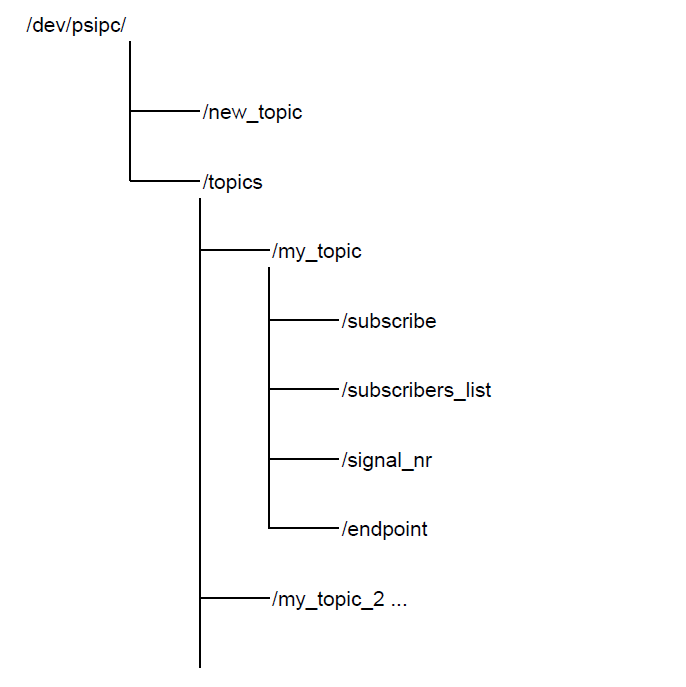
\includegraphics[scale=0.50, center]{assets/psipc_scheme.png}
      \caption{Psipc directory scheme}
      \label{fig: psipc_scheme}
  \end{figure}
\end{center}

The module manages the following device files:
\begin{itemize}
  \item \textbf{new\_topic}: device file responsible of the creation of the topics; whenever the publisher writes here, a new topic is created in the /dev/psipc/topics folder
  \item \textbf{subscribe}: device file that manages the registration of the subscribers, a process can write its PID here to subscribe itself to the topic. Its pid is added to the list of PIDs associated to the topic.
  \item \textbf{subscribers\_list}: device file that manages the list of subscribers pid, a process can retrieve the list of PIDs by reading it
  \item \textbf{signal\_nr}: device file that manages the signal to send to the subscribers, the publisher can write here the numerical value associated to the POSIX signal.
  If the signal hasn't been set, no message is sent to the subscribers.
  \item \textbf{endpoint}: the only device file that can be opened both in read and write mode.
  It is opened in write mode by the publisher that writes here the message, now a signal is sent to all the subscribers to notify them that they can read the message.
  To do so the subscribers open the device file in read mode and retrieve the last message.
  Note that a publisher cannot write a new message until all the notified subscribers have read the previous one.

\end{itemize}

\subsubsection*{Concurrency}
Given the natural tendecy of the files managed by the module to be opened by multiple processes at the same time, syncronization among them is crucial. Moreover, most of the services that the model has to provide to user processes consist in IO operations that generally might noticeably impact overall performance of the module in servicing the users' requests. 

So, after pondering which may be the best fitting solution to deal with processes concurrency, we opted to protect critical sections through Linux \textit{read-write spinlocks} (from now on referred as \textit{rwlock}), since we forsee statistically more reading operations than writing ones: this method allows us to have multiple readers in parallel, especially when the subcribers are invited to go read the new published message in endpoint. Plus, the above-mentioned IO operations are just pseudo IO operations, considering that the module does not perform explicit storaging of data on secondary memory. Furthermore, we expect rather short strings to be written (i.e. PID values take up less than 10 digits at maximum, topics' name should be reasonably short), thus copying data from kernel buffer to user buffer and vice versa should not take long in any case.

So to summarize, we believe that leaving processes spinning for a short period of time but allowing parallel readings is an acceptable compromise.

In the end, the module has one shared \textit{rwlock} to do operations on the general list of all the topics managed by the module. In addition, each topic has 3 \textit{rwlocks} to protect sections modifying respectively the list of subscribers to that particular topic, the signal to send and the published message to be read.
%TODO: check if they're only 3, since maybe we need 4 (even for pid_list)


\section{Project outcomes}

\subsection{Concrete outcomes}
The only artifact is \textbf{psipc\_kmodule.c}, the linux kernel module.
With the makefile is possible to compile it and obtain psipc\_kmodule.ko, the loadable kernel object.

To load the module simply run in the terminal \code{sudo insmod psipc\_kmodule.ko}. By checking the kernel message buffer through \code{dmesg} command, the module has been started up correctly if the new\_topic device major number is printed.

\subsection{Learning outcomes}

Fundamentally we both learned how to develop an out-of-tree linux kernel module.
We both understood that errors at kernel-level are not tolerated and usually result in a system crash, to avoid them is necessary the utmost attention to details.
Another important thing we learned is the use of device files, we managed to let processes in user-space communicate with the module in kernel-space through them.
We understood that each device file acts as an interface meaning that data is not actually stored in the file but copied from the user-space to the kernel-space and viceversa.
Finally we learned how to use spinlocks and atomic operations in order to write concurrent code.

\subsection{Existing knowledge}
\begin{itemize}
  \item \textbf{Advanced Operating Systems (AOS)}: understanding of the linux kernel, IPC mechanisms, device files, POSIX signals, kernel concurrency
  \item \textbf{Architettura dei Calcolatori e Sistemi Operativi (ACSO)}: basic understanding of operating systems
  \item \textbf{Fondamenti di Informatica}: C programming
  \item \textbf{Algoritmi e Principi dell'informatica (API)}: space and time complexity of the algorithms
\end{itemize}

\subsection{Problems encountered}
Since the creation of every device driver file has been delegated to the psipc module running in kernel-mode, \code{root} was the natural owner of those file. Initially, we set the access mode for those file operating mainly on the \textit{Other} permissions to let user processes interact with them. But soon we realised that this method could lead to security issues. In fact, in this way the user creating a new topic or joining one as subscriber had the same privileges of other users in the machine, so giving the read/write permissions to the rightful logical owner (labeled as "other" from the kernel point of view) of the topic meant giving the same permission to anyone else on the system. It was mandatory to think of another way to compartmentalize different users so that a potential threathening one could not interact with another one. For this reason, we decided to let the kernel yields its ownership of the topic directory and files to the user actually requesting it. This brought some problems in identifying the right way to do it from the module code. User-level well known functions for this operation, like \code{chown()}, were out of question, their kernel versions, like \code{ksys\_fchown()}, work just for legacy systems or require the \code{struct file} pointer to the actual file (but opening a file for kernel purposes is no good) and directly calling a system call from kernel code is not advisable too. So, with little to no help for solving this particular issue from the web, we had to learn more about inodes, files as seen by the kernel. Finally, we solved it by directly editing the \code{uid} and \code{gid} fields in the \code{inode} struct associated to the device.

Another minor problem was how to manage input from user-space, we learned to use \code{get\_user()} and \code{put\_user()} functions.

Another challenge was deciding the grain of concurrent accesses to allow within the psipc subsystem. Being all about users and multiple processes interacting with a restricted pool of resources, it is necessary to coordinate them to ensure fairness and well updated data. It's a fact that writing application taking parallellism into consideration is hard, mainly because of the infinite combination of processes schedules and that testing doesn't help much as we would want to. The big difference is that all the resources of a topic are strongly connected, but at the same time the module consist majorly in IO operations that would greatly undermine general performance of the ecosystem if we locked everything. %Add final decision

\section{Honor Pledge}

We pledge that this work was fully and wholly completed within the criteria
established for academic integrity by Politecnico di Milano (Code of Ethics and
Conduct) and represents our original production, unless otherwise cited.\\
We also understand that this project, if successfully graded, will fulfill part B requirement of the
Advanced Operating System course and that it will be considered valid up until
the AOS exam of Sept. 2022. 

\begin{flushright}
Group Students' signatures
\end{flushright}


\end{document}
